\cfoot{Konrad Kelc}
In diesem Kapitel wird die Beschaffung von Informationen über Pflanzen, deren Anbau bzw. Zierfische, sowie deren Haltung behandelt. Homeponics soll dem Benutzer eine möglichst benutzerfreundliche und einfache Art des Anbaus von Pflanzen, sowie der Haltung und Versorgung von Fischen ermöglichen. Deshalb wird dem Nutzer eine Datenbank mit Informationen über verschiedene Arten von Pflanzen und Fischen zur Verfügung gestellt. Die Datenbank ist in der Webapplikation als Lexikon einsehbar. \\  Des Weiteren werden vordefinierte Profile bereitgestellt, welche die optimalen Systemeinstellungen für die verschiedenen Pflanzen und Fische beinhalten. Diese können von dem Benutzer ausgewählt werden. Die Einstellungen werden dann vom System automatisch übernommen, sowie dessen Aktoren angepasst.

\subsubsection{Fische}
Für die Informationen über Fische wurde vom Projektpartner Ponix Systems eine Datenbank zur Verfügung gestellt, welche allgemeine, sowie fachspezifische Informationen über die Haltung und Versorgung einer großen Anzahl an Fischen, darunter auch Zierfische für Aquarien beinhaltet. Aus dieser Datenbank wurden die am meisten verbreiteten, bzw. beliebtesten Zierfische und die relevantesten Informationen über diese ausgewählt.

Folgende Fische wurden für unsere Datenbank ausgewählt:

\begin{itemize}
    \item poecilia reticulata (Guppy)
    \item pterophyllum scalare (Skalar)
    \item paracheirodon innesi (Neonsalmler bzw. Neonfisch)
    \item betta splendens (Siamesischer Kampffisch)
    \item symphysodon aequifasciatus (Diskusbuntbarsch)
    \item mikrogeophagus ramirezi (Schmetterlingsbuntbarsch)
    \item xiphophorus maculatus (Platy)
    \item macropodus opercularis (Makropode)
    \item colisa lalia (Zwergfadenfisch)
    \item puntius tetrazona (Sumatrabarbe)
\end{itemize}

\newpage

Folgende Informationen wurden in unsere Datenbank übernommen:

\begin{itemize}
    \item Name
    \item Bild
    \item Beschreibung
    \item Herkunft
    \item Futter
    \item Wassertemperatur
    \item Besondere Anforderungen
    \item pH-Wert
    \item Mindestanzahl von Tieren
    \item Pflanzen
    \item Bepflanzung
    \item Erreichbares Alter
    \item Benötigt Artenbecken
\end{itemize}

Außer den allgemeinen Informationen wie z.B. Name, Beschreibung, Herkunft etc. gibt es solche, die für die Haltung der Fische relevant sind. Der Punkt, besondere Anforderungen ist besonders hervorzuheben, da einige Fischarten Besonderheiten wie z.B. Unterschlupf, oder Versteckmöglichkeiten bei der Haltung benötigen. Die Mindestanzahl von Tieren ist ebenfalls wichtig, da einige Arten im Schwarm leben bzw. die Gesellschaft von Artgenossen benötigen. Ob eine Art ein Artenbecken benötigt gehört ebenso zu den wichtigsten Informationen, da man bestimmte Arten nicht miteinander Vergesellschaften kann.\\ Der pH-Wert gehört zu den wichtigsten Informationen der Fischhaltung, da verschiedene Fischarten unterschiedliche pH-Werte des Wassers zum Leben benötigen und sie nur einen bestimmten pH-Wert Bereich vertragen. Die Punkte Pflanzen und Bepflanzung sind auch relevant, weil der Benutzer wissen muss, ob und welche Wasserpflanzen man einsetzen kann. Denn bestimmte Fischarten schaden manchen Arten von Pflanzen.\\ \mbox{} \\

\newpage

Ein Beispiel für ein Fischprofil, welches in der Webapp angezeigt wird sieht wie folgt aus:

\begin{figure}[ht]
    \centering
	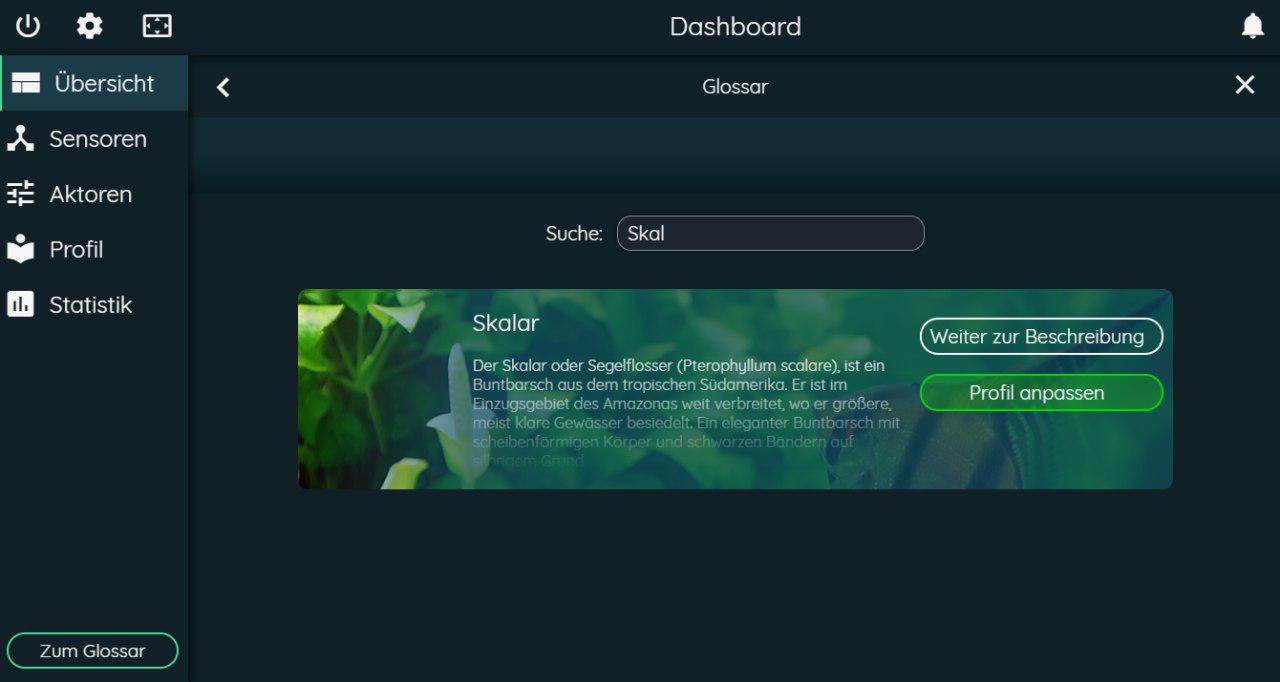
\includegraphics[width=\textwidth]{images/skalar}
    \caption{Skalar}
\end{figure}\mbox{}

\newpage

\subsubsection{Pflanzen}
Bezüglich der Pflanzen werden dem Nutzer Informationen über verschiedene Früchte und Kräuter zur Verfügung gestellt. Für die Datenbank wurden die Sorten gewählt, die sich am besten für Aquaponik bzw. für den Anbau in einer Hydrokultur eignen und ein möglichst schnelles Wachstum bzw. möglichst lange Erntedauer haben. Des Weiteren wurde bei der Auswahl der Sorten darauf geachtet, dass sie den Größenbegrenzungen z.B. in ihrer Wuchshöhe von Homeponics entsprechen.\\Zu den ausgewählten Gemüsesorten gehören unter anderem Tomate, Paprika, oder Kopfsalat. Aus den Kräutern wurden die bekanntesten wie z.B. Basilikum, Oregano, Petersilie genommen. Auch einige auf Sträuchern, oder Stauden wachsende Beeren eignen sich für das Homeponics System. Unter anderem wären hier Erdbeere, Himbeere, Heidelbeere zu nennen.

Die Informationen, welche die Pflanzen betreffend angezeigt werden sind folgende:

\begin{itemize}
    \item Name
    \item Bild
    \item Beschreibung
    \item Keimdauer
    \item Erntedauer
    \item Temperatur
    \item Beleuchtungsdauer
    \item pH-Wert
    \item Wuchshöhe
\end{itemize}

Außer den allgemeinen Informationen gibt es auch hier solche, die für den Anbau und den Benutzer relevant sind. Die Keimdauer der eingesetzten Samen ist wichtig damit der Benutzer weiß, wie lange sie durschnittlich brauchen um zu keimen und der Nutzer nicht unnötig lange wartet, falls es nicht zur Keimung eines Samens kommt. Die Erntedauer ist relevant, damit der Benutzer weiß wie schnell die Pflanzen wachsen bzw. wie lange es dauert bis man sie ernten kann.\\ Die Temperatur gehört zu den wichtigsten Informationen, da die Samen nur in bestimmten Temperaturbereichen keimen bzw. wachsen. Die Beleuchtungsdauer gehört ebenso zu den wichtigsten Informationen, da die Anzahl an Stunden an Licht pro Tag für das Wachstum der Pflanzen wesentlich sind. \\ Wie auch bei den Fischen ist hier der pH-Wert ebenfalls eine der wichtigsten Informationen, da Pflanzen nur in bestimmen pH-Wert-Bereichen wachsen können. Sie vertragen jedoch größere pH-Wert Abweichungen als Fische. 
\newpage 
Die Wuchshöhe ist ebenso relevant, da wie bereits erwähnt die ausgewählte Pflanze für die Maße von Homeponics geeignet sein muss.\\ \mbox{} \\In Aquaponiksystemen erfolgt das Wachstum der Pflanzen um einiges schneller als bei herkömmlichen Anbaumethoden. Da es aber kaum Informationen bzw. Quellen über bestimmte Daten wie z.B. Keimdauer, Erntedauer etc. für Aquaponik gibt, wurden für dieses Projekt größtenteils durschnittliche Werte aus herkömmlichen Indoor und Outdoor Anbaumethoden übernommen.

Ein Beispiel für ein Pflanzenprofil sieht wie folgt aus:

\begin{figure}[ht]
    \centering
	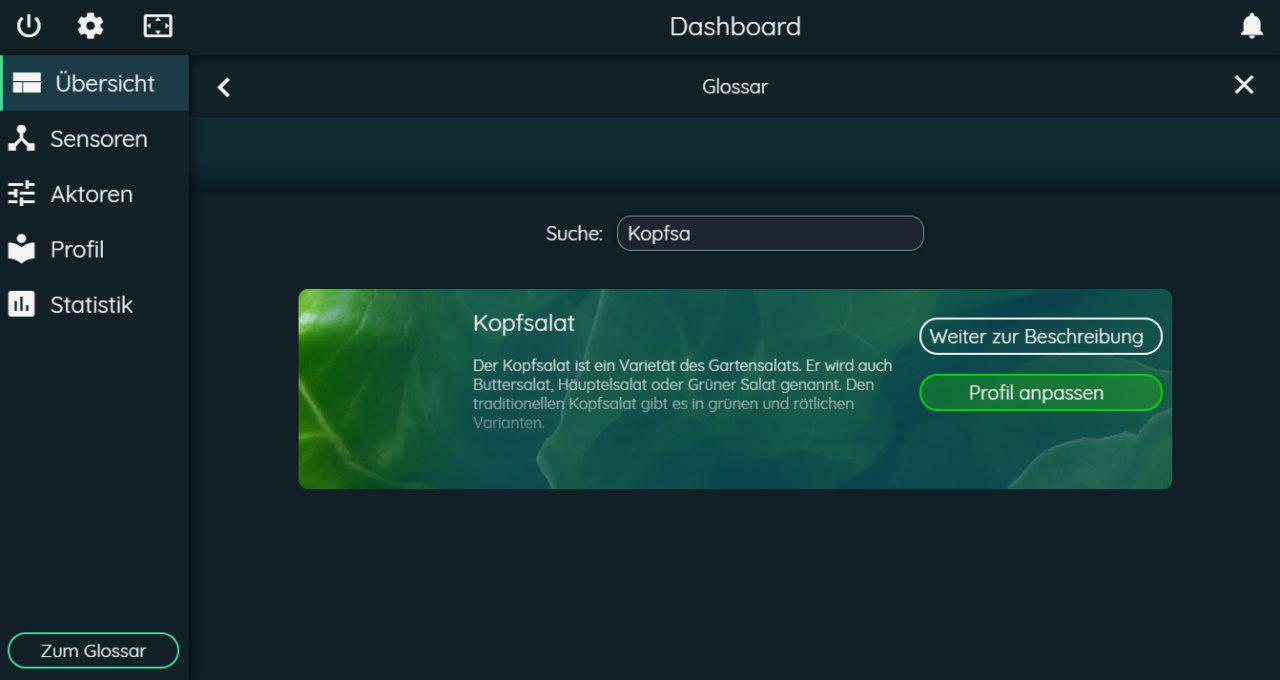
\includegraphics[width=\textwidth]{images/salat}
    \caption{Kopfsalat}
\end{figure}\mbox{}




\afterpage{\blankpage}
\afterpage{\blankpage}